
\phChapterWorksheet{Bonus Puzzle}{Catch Mobimon in the Expedition Zone!}

Take a trip through the \textbf{Expedition Zone} to catch as many Mobimon as you
can! Theres a catch, though: your path through the Expedition Zone has to follow
certain \textbf{path pieces.} Here are the rules:
\begin{enumerate}
\item Two path pieces are adjacent if at least one square in one piece is
  orthogonally (\textbf{not diagonally}) adjacent to at least one square in the
  other piece.
\item You must have a path piece adjacent to the \textbf{starting line}.
\item You must have a path piece adjacent to the \textbf{finish line}.
\item You may not have any breaks in your path. It must be an \textbf{unbroken
    path} of adjacent pieces from start to finish.
\item Your path may cross itself.
\end{enumerate}

You may notice several Mobimon inhabiting the Expedition Zone! These Mobimon are
represented by \textbf{numbers,} and each number is its \textbf{strength.} To
catch a Mobimon, you must

\begin{enumerate}
\item make sure your path goes over that Mobimon, and
\item a piece on that Mobimon must have \textbf{more squares than that Mobimon's
  strength}.
\end{enumerate}

Your score is the \textbf{sum of the strengths of the Mobimon you catch}. The
teams with the two highest scores get \textbf{Victory Points}! Good luck!

\newpage

\phSection{The Expedition Zone}

\begin{center}
  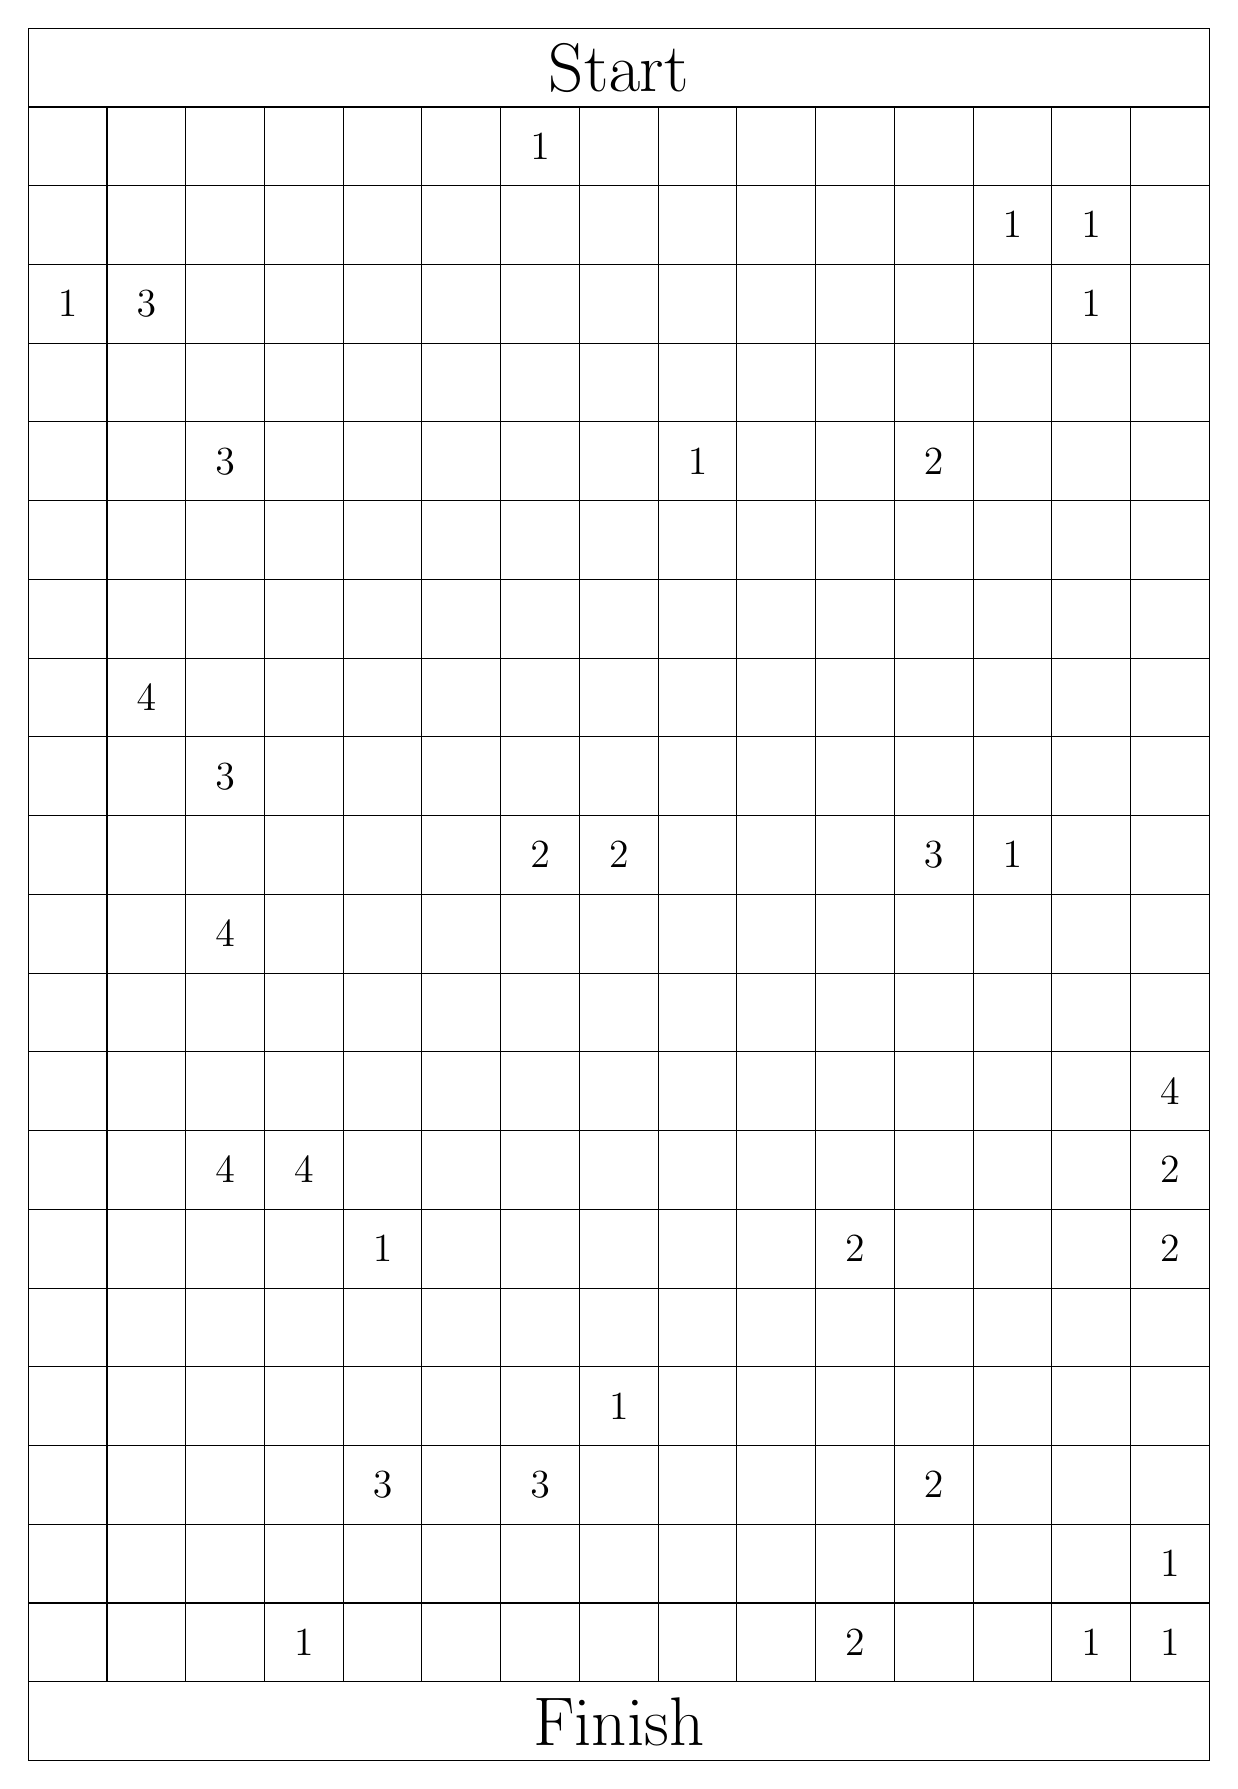
\begin{tikzpicture}
    % start/finish
    \draw[step=10mm] (0,-1) rectangle (15,0);
    \draw[step=10mm] (0,21) rectangle (15, 20);
    \node[font=\Huge] at (7.5, -0.5){Finish};
    \node[font=\Huge] at (7.5, 20.5){Start};

    
    % grid
    \draw[step=10mm] (0,0) grid (15,20);

    
    % nodes - randomly generated by gridgenerator.py
    \tikzstyle{every node}=[font=\Large];
    % run the command:
    % > python gridgenerator.py
    % to generate a new set and copy/paste from gridgen.out (which is a text file
    % despite the unusual extension
    \node at (5mm, 175mm){1};
    \node at (15mm, 125mm){4};
    \node at (15mm, 175mm){3};
    \node at (25mm, 65mm){4};
    \node at (25mm, 95mm){4};
    \node at (25mm, 115mm){3};
    \node at (25mm, 155mm){3};
    \node at (35mm, 5mm){1};
    \node at (35mm, 65mm){4};
    \node at (45mm, 25mm){3};
    \node at (45mm, 55mm){1};
    \node at (65mm, 25mm){3};
    \node at (65mm, 105mm){2};
    \node at (65mm, 195mm){1};
    \node at (75mm, 35mm){1};
    \node at (75mm, 105mm){2};
    \node at (85mm, 155mm){1};
    \node at (105mm, 5mm){2};
    \node at (105mm, 55mm){2};
    \node at (115mm, 25mm){2};
    \node at (115mm, 105mm){3};
    \node at (115mm, 155mm){2};
    \node at (125mm, 105mm){1};
    \node at (125mm, 185mm){1};
    \node at (135mm, 5mm){1};
    \node at (135mm, 175mm){1};
    \node at (135mm, 185mm){1};
    \node at (145mm, 5mm){1};
    \node at (145mm, 15mm){1};
    \node at (145mm, 55mm){2};
    \node at (145mm, 65mm){2};
    \node at (145mm, 75mm){4};
  \end{tikzpicture}
\end{center}

\phSection{Path Pieces}

\begin{center}
  \begin{tikzpicture}
    % monomino
    \draw[step=10mm] (0, -2) grid (1,-1);
    
    % domino
    \draw[step=10mm] (0,0) grid (2,1);
    
    % trominoes
    %% I
    \draw[step=10mm] (0,2) grid (3,3);
    %% L
    \draw[step=10mm] (4,2) grid (6,3);
    \draw[step=10mm] (4,3) grid (5,4);

    % tetraminoes
    %% I
    \draw[step=10mm] (0,5) grid (4,6);
    %% O
    \draw[step=10mm] (5,5) grid (7,7);
    %% T
    \draw[step=10mm] (8,5) grid (11,6);
    \draw[step=10mm] (9,6) grid (10,7);
    %% L
    \draw[step=10mm] (12,5) grid (13,8);
    \draw[step=10mm] (13,5) grid (14,6);
    %% J
    \draw[step=10mm] (0,9) grid (2,10);
    \draw[step=10mm] (1,10) grid (2,12);
    %% Z
    \draw[step=10mm] (3,10) grid (5,11);
    \draw[step=10mm] (4,9) grid (6,10);
    %% S
    \draw[step=10mm] (7,9) grid (9,10);
    \draw[step=10mm] (8,10) grid (10,11);
  \end{tikzpicture}
\end{center}

% Include below for aucTeX integration
%%% Local Variables:
%%% mode: latex
%%% TeX-master: "../mapp-challenge-18-game-book"
%%% End:
